%% Manuscript for The Astronomical Journal -- AASTeX v7.0.2
%% All numerical values come from numbers.tex and tables/*.tex, generated by make_paper_inputs.py
\documentclass[linenumbers]{aastex702}
\usepackage{amsmath}
% AUTO-GENERATED by make_paper_inputs.py from ../results -- do not edit by hand
\newcommand{\NGaia}{321{,}417}
\newcommand{\NFinite}{299{,}746}
\newcommand{\NMS}{218{,}654}
\newcommand{\NMSdec}{212{,}057}
\newcommand{\NSample}{210{,}191}
\newcommand{\NComp}{3{,}381{,}277}
\newcommand{\NMainSample}{1{,}880{,}195}
\newcommand{\NUsedComp}{2{,}235{,}687}
\newcommand{\NSubtiles}{35{,}285}
\newcommand{\NRealOne}{53}
\newcommand{\NOffOne}{2.8}
\newcommand{\EpochMin}{2017.7}
\newcommand{\EpochMax}{2019.5}
\newcommand{\SigSys}{0.23}
\newcommand{\NTrue}{48}
\newcommand{\NSecure}{50}
\newcommand{\NRelNine}{43}
\newcommand{\NFalseSecure}{2.5}
\newcommand{\NCand}{73}
\newcommand{\NRxs}{54}
\newcommand{\NEra}{25}
\newcommand{\NClassAB}{37}
\newcommand{\NClassFL}{7}
\newcommand{\NClassOT}{5}
\newcommand{\NCBinX}{22}
\newcommand{\NCRS}{8}
\newcommand{\NCBY}{6}
\newcommand{\NCBin}{1}
\newcommand{\NCFlare}{3}
\newcommand{\NCXA}{4}
\newcommand{\NCYoung}{2}
\newcommand{\NCCV}{2}
\newcommand{\NCCP}{1}
\newcommand{\NSecureX}{48}
\newcommand{\GBmed}{14.35}
\newcommand{\GBmin}{12.85}
\newcommand{\GBmax}{15.21}
\newcommand{\NUnexplained}{0}
\newcommand{\NNatural}{49}
\newcommand{\NBackground}{1}
\newcommand{\EarthLeakAU}{11{,}300}
\newcommand{\SlimMed}{1.11}
\newcommand{\SlimLo}{0.91}
\newcommand{\SlimHi}{1.60}
\newcommand{\LlimMed}{8.3\times10^{8}}
\newcommand{\EIRPlimMed}{1.7\times10^{18}}
\newcommand{\NConfused}{31}
\newcommand{\NDetected}{50}
\newcommand{\NExcluded}{385}
\newcommand{\NNearComp}{304}
\newcommand{\BarnardL}{5.4\times10^{5}}
\newcommand{\BarnardEIRP}{1.1\times10^{15}}
\newcommand{\BarnardS}{1.34}
\newcommand{\FpopSeven}{2.1\times10^{-2}}
\newcommand{\NpopSeven}{143}
\newcommand{\FpopEight}{6.5\times10^{-4}}
\newcommand{\NpopEight}{4{,}614}
\newcommand{\FpopNine}{2.2\times10^{-5}}
\newcommand{\NpopNine}{134{,}065}
\newcommand{\FpopFloor}{1.4\times10^{-5}}
\newcommand{\NpopFloor}{210{,}191}
\newcommand{\OneInNine}{45{,}000}
\newcommand{\LspmChi}{85.7}
\newcommand{\LspmMu}{68}
\newcommand{\LspmMuErr}{50}
\newcommand{\FrameTieE}{-0.03}
\newcommand{\FrameTieN}{+0.11}
\newcommand{\LspmOffThree}{1.1}
\newcommand{\LspmSigThree}{7}
\newcommand{\PossIO}{20.4}
\newcommand{\PossIE}{19.9}
\newcommand{\PossIIB}{20.9}
\newcommand{\PossIIR}{20.9}
\newcommand{\LspmS}{1.81}
\newcommand{\LspmSep}{0.25}
\newcommand{\LspmRel}{0.985}
\newcommand{\LspmDist}{98}
\newcommand{\LspmMaj}{3.3}
\newcommand{\LspmMin}{1.3}
\newcommand{\StackMS}{11.6}
\newcommand{\StackMSerr}{1.9}
\newcommand{\StackMSNR}{6.2}
\newcommand{\StackMN}{9{,}864}
\newcommand{\StackML}{1.2\times10^{6}}
\newcommand{\StackMMed}{11.8}
\newcommand{\StackMMedSNR}{5.3}
\newcommand{\StackFGKmaxSNR}{2.6}
\newcommand{\NStackStars}{207{,}411}
\newcommand{\ReachFGK}{2.65\times10^{5}}
\newcommand{\DetReachFGK}{1.5\times10^{6}}
\newcommand{\FStackSixFGK}{0.26}
\newcommand{\ReachM}{2.43\times10^{5}}
\newcommand{\DetReachM}{9.4\times10^{5}}
\newcommand{\FStackSixM}{0.24}
\newcommand{\FBratFGK}{0.64}
\newcommand{\FBratM}{0.59}
\newcommand{\TRfloor}{7.1\times10^{-6}}
\newcommand{\ReachEIRP}{4.9\times10^{14}}
\newcommand{\NCutouts}{208{,}573}
\newcommand{\VlassFiftyS}{1.11}
\newcommand{\VlassFiftyEIRP}{6.7\times10^{17}}
\newcommand{\BLratio}{3.2\times10^{5}}
\newcommand{\FluxRatio}{6{,}300}
\newcommand{\NFifty}{26{,}994}
\newcommand{\FFifty}{1.1\times10^{-4}}
\newcommand{\FFiftyHalf}{2.2\times10^{-4}}


\shorttitle{A wideband VLASS technosignature search}
\shortauthors{Croft}
\submitjournal{AJ}
\graphicspath{{figures/}}

\newcommand{\Lnu}{L_\nu}
\newcommand{\WHz}{\mathrm{W\,Hz^{-1}}}

\newcommand{\BLBerkeley}{Breakthrough Listen, University of California, Berkeley, 501 Campbell Hall \#3411, Berkeley, CA 94720, USA}
\newcommand{\seti}{SETI Institute, 339 Bernardo Ave, Suite 200, Mountain View, CA 94043, USA}
\newcommand{\BLOxford}{Breakthrough Listen, University of Oxford, Denys Wilkinson Building, Keble Road, Oxford OX1 3RH, UK}

\begin{document}

\title{A Wideband Technosignature Search of \NSample\ Nearby Main-sequence Stars with the VLA Sky Survey}

\author[orcid=0000-0003-4823-129X, sname='Croft']{Steve Croft} 
\affiliation{\BLOxford}
\affiliation{\BLBerkeley}
\affiliation{\seti}
\email[show]{scroft@berkeley.edu}
\correspondingauthor{Steve Croft}

\begin{abstract}
Searches for radio technosignatures have concentrated on narrowband signals, which are easy to distinguish from natural emission but are only one of many ways a transmitter might radiate. We present a complementary search for excess broadband 2--4\,GHz continuum emission from \NSample\ Gaia DR3 main-sequence stars within 100\,pc, using Epoch~1 of the VLA Sky Survey (VLASS). After propagating each star to the epoch of its VLASS image and calibrating chance alignments with sky-offset catalogs, we find \NSecure\ secure stellar associations (\NFalseSecure\ expected by chance). All but one are explained by known natural emitters---mainly active binaries, flare stars, and X-ray-bright coronae---and the remaining source, near the high-proper-motion M dwarf LSPM~J1943+5337, is shown by multi-epoch VLASS astrometry to be a background source that stays fixed while the star moves. No unexplained detection remains. We place 95\% upper limits on steady 2--4\,GHz emission from every star (median $\Lnu<\LlimMed\,\WHz$; $\Lnu<\BarnardL\,\WHz$ for Barnard's star) and on the fraction of stars hosting a transmitter: $f<\FpopNine$ above $10^9\,\WHz$ and $f<\FpopSeven$ above $10^7\,\WHz$. Stacking \NStackStars\ cutouts in distance shells reveals sub-threshold natural emission from M dwarfs (\StackMS$\pm$\StackMSerr\,$\mu$Jy at 20--40\,pc) but none from FGK stars, and constrains the product of transmitter fraction and power to transmitters 4--6 times fainter than individual non-detections, reaching $f<1$ at $\Lnu\approx\ReachM\,\WHz$ (EIRP $\approx\ReachEIRP$\,W across 2\,GHz). Continuum surveys are $\sim\BLratio$ times less sensitive than targeted narrowband searches to narrow lines, but constrain broadband, modulated, or rapidly drifting signals that narrowband pipelines do not detect.
\end{abstract}

%% UAT concept IDs checked against UAT_list.json (astrothesaurus/UAT, v6.0.0)
\keywords{\uat{Technosignatures}{2128} --- \uat{Search for extraterrestrial intelligence}{2127} --- \uat{Radio continuum emission}{1340} --- \uat{Stellar activity}{1580} --- \uat{Main sequence stars}{1000} --- \uat{Sky surveys}{1464}}

\section{Introduction} \label{sec:intro}

Radio searches for technosignatures have, since their inception, concentrated on narrowband emission \citep[e.g.,][]{Tarter2001}. A signal much narrower than any known natural maser line is an unambiguous marker of technology, and narrowband searches with modern spectrometers reach impressive sensitivity: the Breakthrough Listen (BL) survey of nearby stars \citep{Isaacson2017} placed limits of order $10^{12}$--$10^{13}$\,W on the equivalent isotropic radiated power (EIRP) of drifting narrowband transmitters around 1327 stars within 50\,pc \citep{Enriquez2017,Price2020}, and archival and commensal programs have since extended such searches to many more targets \citep[e.g.,][]{Tremblay2025}. \citet{Painter2025} took a step beyond the drifting-tone paradigm, searching thousands of stars in the BL Green Bank Telescope archive with a kurtosis statistic that flags any non-Gaussian structure within $\sim$3\,kHz-wide spectral blocks rather than matching a template of a single unresolved, Doppler-drifting line---a stepping stone toward searches for broader and more complex signals. Yet narrowband searches sample only a thin slice of the ``cosmic haystack'' \citep{Wright2018}. Terrestrial transmitters are increasingly broadband---spread-spectrum, frequency-hopped, chirped radar and multi-carrier modulations dominate modern usage---and a transmitter whose power is spread over kHz to GHz is effectively invisible to pipelines tuned to Hz-wide drifting lines. Earth's own leakage has shifted from a modest number of powerful broadcast carriers to a vast population of lower-power broadband emitters; \citet{Saide2023} simulated the leakage from the global network of mobile-communication towers as it would appear from nearby stellar systems. \citet{Garrett2026} argued that the aggregate output of such distributed infrastructure would appear to a distant observer as faint, compact continuum emission---a broadband radio technosignature (BRaT)---and, scaling Earth's present aggregate leakage ($\Lnu\sim400\,\WHz$ at L band) linearly with power consumption, estimated $\Lnu\sim4\times10^5\,\WHz$ for a Kardashev Type~I civilization. He proposed a hierarchical search in which wide-field continuum surveys identify compact sources coincident with nearby stars and very long baseline interferometry (VLBI) then tests them for high brightness temperature, negligible polarization, non-uniform spectra, scintillation, and co-motion with the host star, and noted that existing surveys can already place the first constraints on BRaT prevalence.

Wide-area radio continuum surveys offer a complementary probe. They integrate the total power in a broad band irrespective of modulation, drift rate, or bandwidth, and they cover a large fraction of the sky to a uniform depth, so that every star in a volume-limited sample is observed. The cost is that a stellar continuum source is not intrinsically artificial: active stars emit gyrosynchrotron and coherent radio emission \citep{GudelBenz1993,Callingham2021,Vedantham2022}, and the overwhelming majority of mJy radio sources are extragalactic and can align with a foreground star by chance. A continuum technosignature search is therefore a search for \emph{unexplained} radio emission, and its power lies in the care with which natural explanations and chance alignments are eliminated.

Here we carry out the first stage of such a search, for an entire volume-limited stellar sample, using Epoch~1 of the VLA Sky Survey \citep[VLASS;][]{Lacy2020}, which covers the sky north of $\delta=-40^\circ$ at 2--4\,GHz with $\sim$2.5$''$ resolution and $\sim$0.12--0.15\,mJy\,beam$^{-1}$ noise, together with Gaia DR3 \citep{GaiaMission,GaiaDR3}. We cross-match all main-sequence stars within 100\,pc against the VLASS Quick Look component catalog \citep{Gordon2020,Gordon2021}, quantify chance alignments with offset catalogs, classify every association, follow up the one unexplained source with archival optical imaging and multi-epoch VLASS astrometry, derive limits on individual stars and on the population, and stack the images of all individually undetected stars. Section~\ref{sec:data} describes the data, Section~\ref{sec:methods} the methods, Section~\ref{sec:results} the results, and Section~\ref{sec:discussion} compares them with narrowband searches and with broadband leakage benchmarks. All code and data needed to reproduce this work are publicly available (Section~\ref{sec:data_avail}).

\section{Data} \label{sec:data}

\subsection{Nearby main-sequence stars from Gaia DR3} \label{sec:gaia}

We selected the \NGaia\ Gaia DR3 sources with parallax $\varpi>10$\,mas, $\varpi/\sigma_\varpi>10$, and $\delta>-45^\circ$. Of these, \NFinite\ have a $G_{BP}-G_{RP}$ color. We defined the main sequence empirically as the iteratively clipped median absolute magnitude $M_G$ in 0.1\,mag bins of $G_{BP}-G_{RP}$, after coarse cuts removing white dwarfs and giants, and retained stars within $-1.5<\Delta M_G<+1.0$\,mag of this ridge. The asymmetric window keeps unresolved binaries (up to 0.75\,mag over-luminous for equal-mass pairs) and excludes the white-dwarf sequence and the spurious faint sources below the main sequence that are known to contaminate Gaia nearby-star samples \citep{Smart2021}. This leaves \NMS\ stars, of which \NMSdec\ lie at $\delta>-41^\circ$ and \NSample\ fall within the VLASS Epoch~1 footprint. We divide the sample at $G_{BP}-G_{RP}=1.84$, close to the K7/M0 boundary \citep{Pecaut2013}, into FGK stars and M dwarfs.

\subsection{VLASS Epoch 1} \label{sec:vlass}

VLASS Epoch~1 was observed in two halves (1.1 and 1.2) between \EpochMin\ and \EpochMax\ \citep{Lacy2020}. We use the CIRADA Quick Look (QL) component catalog \citep{Gordon2020,Gordon2021}, which contains \NComp\ components extracted with PyBDSF \citep{Mohan2015} from \NSubtiles\ $1\,\mathrm{deg}^2$ QL images. We use all \NUsedComp\ non-duplicate components with a fitted Gaussian (not only the \NMainSample\ in the recommended ``main sample''), so that faint and low-quality components near stars are also considered. QL flux densities are systematically low by $\sim$10--15\% \citep{Gordon2021}; we divide all catalog and image flux densities by 0.87. The QL astrometric accuracy is $\lesssim1''$; we calibrate it empirically below. The CIRADA catalog also lists, for each component, the distance to the nearest NVSS \citep{Condon1998} and FIRST \citep{Becker1995,Helfand2015} source, which we use to test whether radio sources move with their candidate host stars. For image-based analyses we retrieved QL and Single Epoch images for epochs 1--3 from the Canadian Astronomy Data Centre (CADC).

\subsection{Ancillary data} \label{sec:ancillary}

For every star with a VLASS component within 2.5$''$ we retrieved the nearest ROSAT 2RXS \citep[within 40$''$;][]{Boller2016} and eROSITA eRASS1 \citep[within 20$''$;][]{Merloni2024} X-ray sources via VizieR \citep{Ochsenbein2000}, and SIMBAD \citep{Wenger2000} identifications and object types. For the one unexplained candidate we also used Digitized Sky Survey (POSS-I and POSS-II) plates and Pan-STARRS1 images and catalogs \citep{Chambers2016,Flewelling2020}.

\section{Methods} \label{sec:methods}

\subsection{Epoch propagation and cross-matching} \label{sec:xmatch}

Many nearby stars move by several arcseconds between the Gaia reference epoch (J2016.0) and the VLASS observations. We assigned each star to the QL image whose center is nearest, and propagated its position linearly to that image's observation date; for the final reliability analysis each star--component pair was re-propagated to the date of the image in which the component was measured. Parallactic displacement ($\le0.55''$, for Barnard's star) was neglected. We then found all components within 10$''$ of each star.

To measure the rate of chance alignments directly, we repeated the match ten times after displacing every star by 3$'$ in a random direction. Figure~\ref{fig:sep} compares the separation distributions: there are \NRealOne\ star--component pairs within 1$''$, against \NOffOne\ per offset realization, while beyond $\sim$2.5$''$ the two distributions agree.

\begin{figure}
\centering
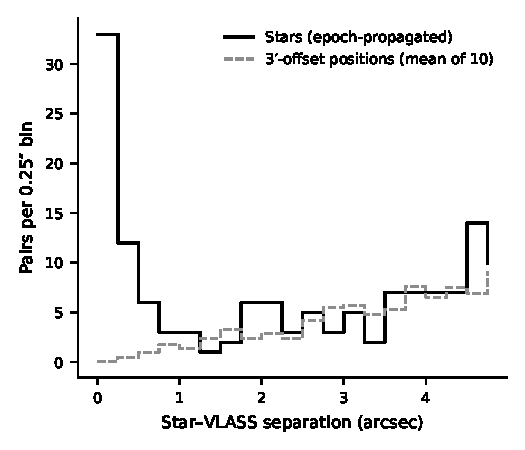
\includegraphics[width=0.6\textwidth]{vlass_separation_histogram.pdf}
\caption{Separations between epoch-propagated stars and VLASS components (solid) compared with the mean of ten 3$'$-offset realizations (dashed). The excess within 1$''$ is due to genuine stellar associations; beyond $\sim$2.5$''$ the two distributions agree.\label{fig:sep}}
\end{figure}

\subsection{Positional reliability} \label{sec:reliability}

We modeled the separations $r_i$ of all pairs within $R_{\max}=10''$ as a mixture of genuine associations, with a two-dimensional Gaussian offset distribution, and background sources with a uniform surface density $\lambda$ per star fixed from the offset catalogs:
\begin{equation}
p_{\rm true}(r_i)=f\,\frac{r_i}{\sigma_i^2}\exp\!\left(-\frac{r_i^2}{2\sigma_i^2}\right),\qquad
p_{\rm bg}(r_i)=2\pi\lambda r_i,\qquad
\sigma_i^2=\sigma_{{\rm cat},i}^2+\sigma_{\rm sys}^2,
\end{equation}
where $\sigma_{{\rm cat},i}$ is the per-axis catalog positional error and $f$ the fraction of stars genuinely detected. Maximizing the extended likelihood gives $\sigma_{\rm sys}=\SigSys''$ per axis and $\approx$\NTrue\ genuine associations. The reliability of each pair is $R_i=p_{\rm true}/(p_{\rm true}+p_{\rm bg})$. We call pairs with $R>0.5$ secure: there are \NSecure\ (\NRelNine\ with $R>0.9$), among which $\sum(1-R)=\NFalseSecure$ chance alignments are expected.

\subsection{Classification of associations} \label{sec:classify}

Each star with $R>0.05$ was classified in the following order of precedence: cataclysmic variable; magnetic chemically peculiar star; RS~CVn binary; young star (T~Tauri or young stellar object); BY~Dra variable (all from SIMBAD object types); binary or over-luminous star (SIMBAD eclipsing or spectroscopic binary, Gaia non-single-star flag, RUWE\,$>1.4$, or $\Delta M_G<-0.5$\,mag), with or without an X-ray counterpart; flare star; X-ray-active single star; otherwise unexplained. For stars with X-ray counterparts we computed $\log(L_X/\Lnu)$, using the eRASS1 0.2--2.3\,keV flux where available and otherwise the 2RXS count rate with a coronal energy conversion factor of $6\times10^{-12}$\,erg\,cm$^{-2}$\,count$^{-1}$, for comparison with the G\"udel--Benz relation, $L_X/\Lnu\approx10^{15.5}$\,Hz \citep{GudelBenz1993}.

Unexplained associations were then tested for being background sources. (1) A radio source that coincides with an NVSS or FIRST source at the VLASS position, although the star has since moved by more than twice that offset, is stationary and therefore background. (2) For the one source surviving this test we compared archival optical images taken when the star was displaced from the radio position, and measured the radio position in three VLASS epochs relative to the star's Gaia track (Section~\ref{sec:lspm}).

\subsection{Limits on individual stars} \label{sec:limits_method}

For a star without a secure association we adopt a 95\%-completeness flux-density limit
\begin{equation}
S_{\rm lim}=\frac{(5+1.645)\,\sigma_{\rm img}}{0.87},
\end{equation}
where $\sigma_{\rm img}$ is the mean island rms of the star's QL image and 5$\sigma$ is the PyBDSF detection threshold. If an unrelated component lies within 3$''$ (\NConfused\ stars) the limit is raised to that component's flux density; for the \NDetected\ securely detected stars, the limit on any artificial component is the measured flux density plus 1.645$\sigma$. The spectral luminosity limit is $\Lnu^{\rm lim}=4\pi d^2S_{\rm lim}$ and, for a transmitter whose power is spread uniformly over the 2--4\,GHz band, ${\rm EIRP}_{\rm lim}=\Lnu^{\rm lim}\times2$\,GHz. A narrowband transmitter anywhere in the band contributes its total power divided by the 2\,GHz bandwidth to the continuum flux density, so the same EIRP limit applies to any in-band signal regardless of its width.

\subsection{Population limits} \label{sec:pop_method}

If a fraction $f$ of stars host a transmitter with $\Lnu\ge L_T$, and $N_{\rm eff}(L_T)$ stars have individual limits below $L_T$, the expected number of detections is $fN_{\rm eff}$. With no unexplained detections, the 95\% upper limit is $f<3.0/N_{\rm eff}(L_T)$. Securely detected stars count only for $L_T$ above their measured luminosity. Because each VLASS position is observed for only a few seconds in a single epoch, $f$ is strictly a limit on the product of the fraction of stars hosting a transmitter and its duty cycle.

\subsection{Image stacking} \label{sec:stack_method}

To probe emission below the single-star threshold we extracted $41''\times41''$ QL cutouts centered on each star's epoch-propagated position from CADC, using one multi-extension request per image. We excluded the securely detected and confused stars and the \NNearComp\ further stars with any non-associated catalog component within 10$''$, leaving \NStackStars\ stars in twelve stacks: six distance shells (0--10, 10--20, 20--40, 40--60, 60--80, and 80--100\,pc), each split into FGK and M stars. For each cutout we measured a robust (median absolute deviation) noise $\sigma_i$ from pixels more than 8$''$ from the center, discarding the few cutouts with $\sigma_i$ more than five times the median (sidelobe-dominated regions). The primary statistic is the inverse-variance-weighted mean spectral luminosity
\begin{equation}
\langle\Lnu\rangle=\frac{\sum_i w_i\,4\pi d_i^2 S_i}{\sum_i w_i},\qquad w_i=\left(4\pi d_i^2\sigma_i\right)^{-2},
\end{equation}
evaluated at the central pixel and corrected for the mean peak loss from sub-pixel centering (a factor $\approx0.93$). We also formed flux-density means and medians. The stacked image at 10--18$''$ from the center provides an empirical null: we subtract its mean and adopt the larger of its scatter and the formal error. As robustness tests we compared halves of the sky ($\alpha<180^\circ$ and $\ge180^\circ$) and recomputed the means after removing the brightest 1\% of central pixels, correcting for the bias this truncation introduces by applying the same trimming at null-ring pixels.

A mean stack constrains the product of the fraction of stars with a transmitter and its power: $f\,L_T\le\langle\Lnu\rangle_{95}$, where $\langle\Lnu\rangle_{95}$ is the one-sided 95\% upper limit. Because individually detected stars are excluded, each shell is truncated at a luminosity threshold that rises as $d^2$. We therefore combine, for each $L_T$, only shells in which a transmitter of that power would \emph{not} have been individually detected (5th percentile of the per-star limits above $L_T$); more powerful transmitters are covered by the individual limits of Section~\ref{sec:pop_method}.

\section{Results} \label{sec:results}

\subsection{Radio-detected stars are natural emitters} \label{sec:matches}

Table~\ref{tab:matches} lists the \NSecure\ secure associations, and Figure~\ref{fig:cmd} shows them on the color--magnitude diagram. Of the \NCand\ stars with a VLASS component within 2.5$''$, \NRxs\ have a 2RXS and \NEra\ an eRASS1 counterpart; the chance of a random 2RXS source within 40$''$ is $\sim10^{-3}$. Among the secure associations, \NClassAB\ are active binaries (\NCBinX\ binary or over-luminous stars with X-ray counterparts, \NCRS\ RS~CVn systems, \NCBY\ BY~Dra variables, and \NCBin\ binary without X-ray detection), \NClassFL\ are flare stars or X-ray-active single stars, and \NClassOT\ are other known radio emitters: two young stars, two cataclysmic variables (including AE~Aqr), and the magnetic Ap star $\alpha^2$~CVn. The X-ray-detected stars have $\log(L_X/\Lnu)=\GBmin$--\GBmax\ (median \GBmed), $\sim$1\,dex radio-bright relative to the G\"udel--Benz relation, as expected for a radio flux-limited selection and consistent with the radio-loud tail of active stars \citep{Vedantham2022}. The remaining secure association is discussed next. Two lower-reliability unexplained matches, LP~732-30 and 2MASS~J14223872+0646143, are stationary in NVSS and FIRST respectively and are background sources.

\begin{figure}
\centering
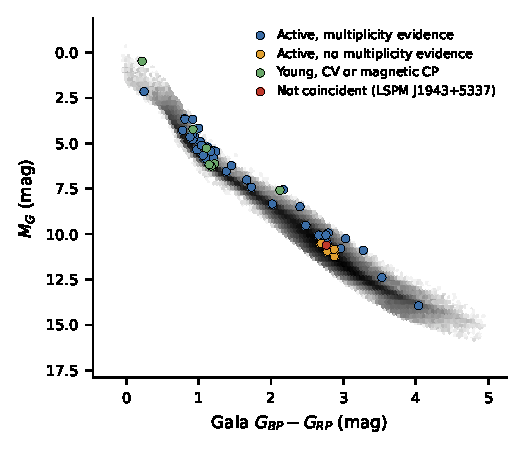
\includegraphics[width=0.6\textwidth]{vlass_detections_cmd.pdf}
\caption{Color--magnitude diagram of the \NSample\ sample stars (grey) with the \NSecure\ secure associations colored by classification: active binaries (RS~CVn, BY~Dra, and other binary or over-luminous stars; blue), flare or X-ray-active single stars (orange), other natural emitters (young stars, cataclysmic variables, and a magnetic chemically peculiar star; green), and the background source near LSPM~J1943+5337 (red).\label{fig:cmd}}
\end{figure}

\setlength{\tabcolsep}{2.5pt}
\begin{deluxetable*}{lrrrrrrrrrcrl}
\tabletypesize{\scriptsize}
\tablecaption{VLASS Epoch 1 components securely associated (reliability $R>0.5$) with \NSecure\ main-sequence stars within 100\,pc.\label{tab:matches}}
\tablehead{\colhead{Name} & \colhead{Gaia DR3} & \colhead{$d$} & \colhead{$G_{BP}-G_{RP}$} & \colhead{$\Delta M_G$} & \colhead{RUWE} & \colhead{Sep.} & \colhead{$R$} & \colhead{$S_{3\,\rm GHz}$} & \colhead{$\log L_\nu$} & \colhead{X-ray} & \colhead{$\log\frac{L_X}{L_\nu}$} & \colhead{Class} \\
\colhead{} & \colhead{} & \colhead{(pc)} & \colhead{(mag)} & \colhead{(mag)} & \colhead{} & \colhead{($''$)} & \colhead{} & \colhead{(mJy)} & \colhead{(W\,Hz$^{-1}$)} & \colhead{} & \colhead{(Hz)} & \colhead{}}
\startdata
{G 9-38B} & 660597997697274752 & 5.1 & 4.04 & +0.04 & 3.54 & 0.88 & 0.820 & 4.99 & 7.19 & E & 13.23 & B+X \\
{BD+19 5116A} & 2824770686019003904 & 6.3 & 2.66 & -0.47 & 1.32 & 0.29 & 0.980 & 1.30 & 6.78 & R & 15.07 & Fl \\
{V374 Peg} & 1893189736896880640 & 9.1 & 2.87 & -0.37 & 1.17 & 0.64 & 0.864 & 1.70 & 7.23 & R & 14.18 & Fl \\
{CW UMa} & 758200712885953280 & 13.4 & 2.69 & -0.12 & 1.14 & 0.24 & 0.983 & 2.29 & 7.69 & RE & 13.89 & Fl \\
{alf For B} & 5059349158319689344 & 14.1 & 1.11 & -0.09 & 2.85 & 0.66 & 0.739 & 5.21 & 8.09 & RE & 14.44 & B+X \\
{CD-38 11343B} & 5970189504209690496 & 15.7 & 2.96 & -0.69 & 1.25 & 0.92 & 0.732 & 2.23 & 7.82 & RE & 14.98 & B+X \\
{1RXS J055641.0-101837} & 2999254213453678720 & 15.9 & 2.78 & +0.05 & 1.27 & 0.51 & 0.948 & 1.05 & 7.50 & RE & 13.60 & X \\
{G 249-36} & 1005873614080407296 & 16.3 & 2.87 & +0.03 & 1.36 & 0.16 & 0.991 & 9.68 & 8.49 & R & 12.93 & X \\
{HD 43162C} & 2913314288686472576 & 16.7 & 2.78 & -0.37 & 1.41 & 0.33 & 0.980 & 3.39 & 8.05 & E & 13.94 & B+X \\
{HD 283750} & 151650076838458112 & 17.4 & 1.38 & -0.24 & 1.81 & 0.32 & 0.981 & 3.41 & 8.09 & R & 14.68 & BY \\
{LQ Hya} & 5739942011185493888 & 18.3 & 1.14 & +0.09 & 1.07 & 0.08 & 0.989 & 1.52 & 7.78 & RE & 15.01 & BY \\
{Ross 776} & 1851868127125091840 & 19.7 & 2.79 & -1.00 & 19.19 & 0.28 & 0.985 & 3.44 & 8.20 & R & 13.87 & B+X \\
{BD+55 1823} & 1429437378934511616 & 20.1 & 2.17 & -1.40 & 39.08 & 0.21 & 0.988 & 1.85 & 7.95 & R & 14.49 & B+X \\
{sig CrB A} & 1328866562170960512 & 22.7 & 0.81 & -0.92 & 1.22 & 0.21 & 0.989 & 4.14 & 8.41 & R & 15.14 & B+X \\
{BF Lyn} & 812477352773908608 & 23.4 & 1.24 & -0.93 & 0.95 & 0.37 & 0.976 & 1.19 & 7.89 & RE & 15.18 & BY \\
{[R78b] 233} & 3274291270411229056 & 26.8 & 3.03 & -1.46 & 1.50 & 0.23 & 0.986 & 1.91 & 8.21 & RE & 13.69 & B+X \\
{V478 Lyr} & 2042389925739687808 & 27.1 & 0.98 & -0.08 & 1.21 & 0.18 & 0.990 & 3.15 & 8.44 & R & 14.61 & RS \\
{StKM 1-497} & 3205094369407459456 & 27.8 & 2.12 & -1.24 & 22.86 & 0.54 & 0.921 & 1.64 & 8.18 & RE & 14.26 & Y \\
{PW And} & 2860839993168687872 & 28.3 & 1.17 & +0.08 & 0.99 & 0.21 & 0.988 & 1.97 & 8.28 & R & 14.67 & RS \\
{HD 124498A} & 6298167775459045632 & 29.0 & 1.73 & -0.28 & 16.36 & 0.33 & 0.977 & 0.92 & 7.97 & RE & 14.60 & B+X \\
{2MASS J17022950+1341015} & 4544627976777952640 & 30.5 & 3.53 & -0.60 & 5.27 & 0.85 & 0.764 & 1.55 & 8.24 & \nodata & \nodata & B \\
{alf02 CVn} & 1517698716348324992 & 30.6 & 0.22 & -1.39 & 8.42 & 0.21 & 0.988 & 1.77 & 8.30 & R & 13.52 & CP \\
{HD 166181} & 4590455518346609792 & 32.1 & 0.92 & -0.38 & 8.85 & 0.09 & 0.991 & 1.16 & 8.15 & R & 15.21 & RS \\
{GS Leo} & 589720969909457792 & 35.4 & 1.06 & -0.14 & 1.64 & 0.10 & 0.990 & 1.93 & 8.46 & RE & 14.34 & BY \\
{IZ Boo} & 1484942233437321728 & 36.0 & 2.40 & -1.19 & 1.38 & 0.48 & 0.948 & 2.07 & 8.51 & R & 13.72 & B+X \\
{HD 22403} & 69443337640657536 & 36.6 & 0.92 & -0.96 & 1.35 & 0.29 & 0.984 & 2.61 & 8.62 & R & 14.98 & Y \\
{V376 Cep} & 2299477768899190400 & 39.9 & 0.91 & -0.80 & 1.03 & 0.42 & 0.965 & 2.82 & 8.73 & R & 14.74 & RS \\
{NQ Com} & 3955187043030098176 & 40.5 & 1.67 & -0.51 & 1.41 & 0.58 & 0.919 & 0.89 & 8.24 & RE & 14.42 & BY \\
{HD 143937} & 6243343170769568128 & 42.9 & 1.10 & -0.74 & 1.07 & 0.32 & 0.981 & 2.34 & 8.71 & RE & 14.53 & B+X \\
{HD 195434A} & 4245659976227848704 & 45.1 & 1.20 & -0.47 & 1.39 & 0.14 & 0.988 & 1.37 & 8.52 & R & 14.69 & B+X \\
{V402 Hya} & 5756823564825367936 & 47.5 & 1.17 & -0.71 & 5.06 & 0.40 & 0.970 & 3.04 & 8.91 & RE & 14.35 & BY \\
Gaia DR3 3821318547411001728 & 3821318547411001728 & 49.0 & 2.48 & -0.43 & 7.77 & 0.11 & 0.991 & 1.53 & 8.64 & RE & 13.45 & B+X \\
{HD 200391} & 1845206534070618624 & 50.5 & 0.81 & -0.94 & 0.90 & 0.65 & 0.906 & 2.85 & 8.94 & R & 14.72 & RS \\
{HD 25284} & 4888246251178417024 & 50.6 & 1.45 & -0.75 & 11.93 & 0.60 & 0.896 & 1.77 & 8.73 & RE & 14.35 & B+X \\
{EV Dra} & 1403766939225964288 & 57.5 & 0.94 & -0.69 & 0.92 & 0.29 & 0.984 & 1.80 & 8.85 & R & 14.48 & RS \\
{UCAC4 747-046156} & 860453786736413568 & 57.7 & 3.28 & -1.50 & 1.23 & 0.24 & 0.986 & 2.03 & 8.91 & R & 12.85 & B+X \\
{HD 79551} & 818854107897169024 & 60.1 & 0.88 & -0.33 & 1.22 & 0.56 & 0.908 & 1.29 & 8.75 & R & 14.61 & X \\
{BD+47 4087} & 1942527533757602176 & 60.3 & 1.04 & -0.60 & 0.93 & 0.28 & 0.984 & 1.21 & 8.72 & R & 14.47 & B+X \\
{HD 295290} & 3105605708307826944 & 60.5 & 1.02 & -0.74 & 1.10 & 0.18 & 0.990 & 6.88 & 9.48 & RE & 13.93 & B+X \\
{BD+18 1512} & 3361628369521591808 & 61.7 & 1.03 & -0.73 & 36.41 & 0.14 & 0.991 & 10.50 & 9.68 & RE & 13.69 & B+X \\
{HD 8358} & 2534358706998049792 & 62.3 & 1.00 & -1.38 & 0.95 & 0.30 & 0.983 & 4.44 & 9.31 & R & 14.32 & RS \\
{RZ Cas} & 541801332594262912 & 65.3 & 0.25 & +0.19 & 0.93 & 0.24 & 0.987 & 3.36 & 9.23 & R & 14.12 & B+X \\
{XY UMa} & 1023682919309621632 & 67.9 & 1.12 & -0.81 & 0.98 & 0.41 & 0.968 & 1.85 & 9.01 & R & 14.07 & RS \\
{1RXS J204412.7+312642} & 1859797431337296384 & 68.5 & 2.02 & -0.16 & 28.62 & 0.31 & 0.980 & 3.17 & 9.25 & R & 13.03 & B+X \\
{HD 101207B} & 767786259553138816 & 81.1 & 0.92 & -0.65 & 2.07 & 0.19 & 0.986 & 0.82 & 8.81 & R & 14.52 & B+X \\
{BD+08 102} & 2750199780197751936 & 81.1 & 1.11 & -0.69 & 11.62 & 0.09 & 0.992 & 2.08 & 9.21 & R & 14.12 & CV \\
{BD+66 1664} & 2210120493272273920 & 89.4 & 0.92 & -1.50 & 1.10 & 0.40 & 0.970 & 1.92 & 9.26 & R & 14.40 & B+X \\
{AE Aqr} & 4226332451596335616 & 91.6 & 1.22 & -0.20 & 1.14 & 0.29 & 0.983 & 2.97 & 9.47 & R & 14.28 & CV \\
{HD 156848B} & 4108078979665915648 & 93.4 & 0.78 & -0.15 & 0.68 & 0.69 & 0.781 & 1.33 & 9.14 & RE & 14.30 & X \\
{LSPM J1943+5337} & 2137474969751117312 & 97.6 & 2.77 & -0.24 & 1.15 & 0.25 & 0.985 & 2.08 & 9.37 & \nodata & \nodata & BG \\
\enddata
\tablecomments{Sorted by distance. Separation at the epoch of the component's VLASS image. $S_{3\,\rm GHz}$ is the catalogued total flux density divided by 0.87 (Quick Look flux-scale correction). X-ray: R = ROSAT 2RXS, E = eRASS1. Class: B+X binary/over-luminous with X-ray detection; RS = RS~CVn; BY = BY~Dra; B = binary/over-luminous; Fl = flare star; X = X-ray-active single star; Y = young star; CV = cataclysmic variable; CP = magnetic chemically peculiar star; BG = background source (Section~\ref{sec:lspm}). A machine-readable version with all columns is provided in the reproducibility package.}
\end{deluxetable*}


\subsection{LSPM J1943+5337: a background source} \label{sec:lspm}

The radio component \LspmSep$''$ from the M dwarf LSPM~J1943+5337 ($d=\LspmDist$\,pc; $R=\LspmRel$) has a 3\,GHz flux density of \LspmS\,mJy and no X-ray counterpart, and the star has no SIMBAD activity classification; it is the only secure association without a natural explanation. Its catalogued deconvolved size, $\LspmMaj''\times\LspmMin''$, already argued for an extragalactic source. The star moves north at 153\,mas\,yr$^{-1}$, so in POSS-I (1953) it lay 9.8$''$ and in POSS-II (1989--1992) $\approx4''$ from the radio position. No optical source is present at the radio position on these plates to $g\gtrsim\PossIO$ and $r\gtrsim\PossIE$ (POSS-I) and $B_J,R_F\gtrsim\PossIIB$ (POSS-II; Figure~\ref{fig:lspm_optical}). Because only $\sim$30\% of mJy radio sources have optical counterparts even at $r\approx22$ \citep{Ivezic2002}, and fewer at plate depth \citep{deVries2004}, this non-detection is weak evidence on its own. The archival imaging also reveals a common-proper-motion companion, Gaia~DR3~2137474969749746048, 3.4$''$ south of the star, whose faintness and colors suggest a cool white dwarf.

\begin{figure*}
\centering
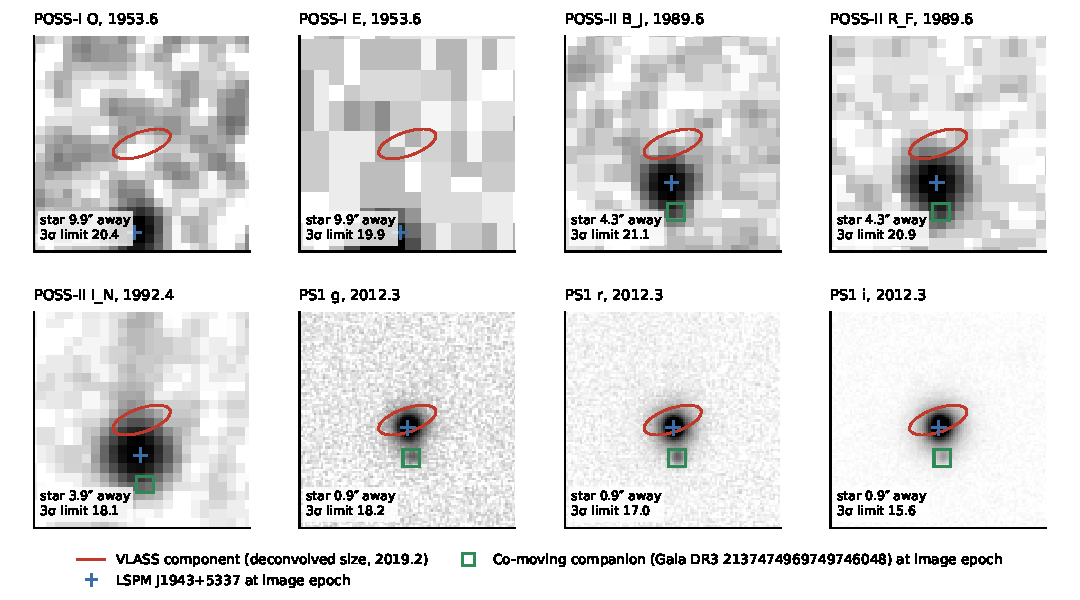
\includegraphics[width=0.95\textwidth]{lspm1943_archival_imaging.pdf}
\caption{Archival optical images ($24''\times24''$, north up, east left) around the VLASS component near LSPM~J1943+5337 (red ellipse: deconvolved size). The blue cross marks the star and the green cross its co-moving companion at each image epoch. The star was displaced by 9.8$''$ (POSS-I) and $\approx4''$ (POSS-II) from the radio position; 3$\sigma$ limits at the radio position are given in each panel. At the Pan-STARRS1 epoch the star is only 0.8$''$ away and dominates the light.\label{fig:lspm_optical}}
\end{figure*}

The decisive test is astrometric. Table~\ref{tab:lspm} and Figure~\ref{fig:lspm_vlass} show the radio position in VLASS epochs 1.2, 2.2, and 3.2, after tying each image to five compact reference sources; the reference frame agrees with Gaia to within $(\Delta\alpha^*,\Delta\delta)=(\FrameTieE'',\FrameTieN'')$ for the secure stellar associations. The source is detected at a steady $\approx$1\,mJy\,beam$^{-1}$ in every epoch while the star moved $\approx$0.8$''$ north; by 2024.4 the radio source lies $\LspmOffThree''$ from the star (\LspmSigThree$\sigma$ in declination), and a model in which the emission tracks the star is excluded with $\chi^2=\LspmChi$ for three degrees of freedom. LSPM~J1943+5337 is therefore a chance alignment with a background source. No unexplained secure association remains in the sample.

\begin{figure*}
\centering
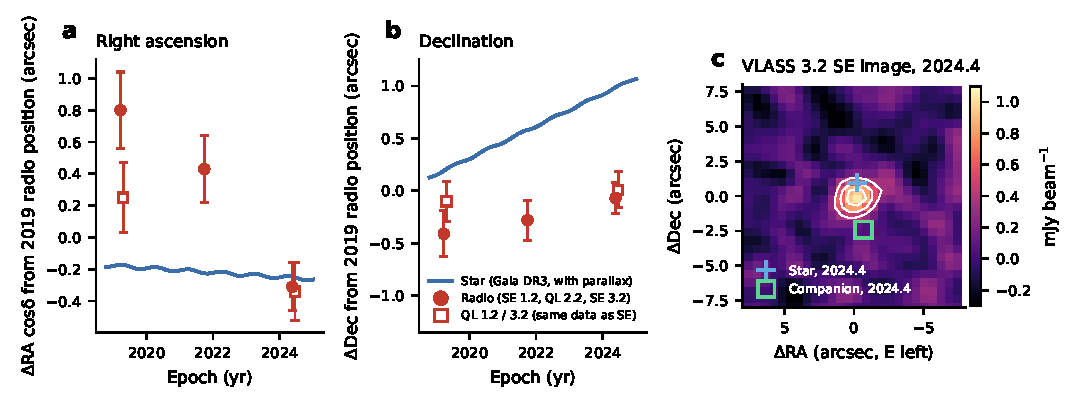
\includegraphics[width=0.95\textwidth]{lspm1943_vlass_multiepoch_astrometry.pdf}
\caption{(a) Declination offset of the radio source near LSPM~J1943+5337 relative to its Epoch 1 catalog position (red), in a frame tied to compact reference sources, compared with the Gaia track of the star (blue). Filled symbols are independent epochs; open squares are Quick Look images sharing data with the Single Epoch images. (b) VLASS 3.2 Single Epoch image (2024.4) with contours at 3, 5, and 7 times the rms; the star (cross) has moved 1.1$''$ from the radio source.\label{fig:lspm_vlass}}
\end{figure*}

\begin{deluxetable}{lrrrrrrr}
\tablecaption{Multi-epoch VLASS astrometry of the radio source near LSPM~J1943+5337.\label{tab:lspm}}
\tablehead{\colhead{Image} & \colhead{Epoch} & \colhead{$S_{\rm peak}$} & \colhead{SNR} & \colhead{$\Delta\alpha^*$} & \colhead{$\Delta\delta$} & \colhead{$\Delta\alpha^*_\star$} & \colhead{$\Delta\delta_\star$} \\
\colhead{} & \colhead{(yr)} & \colhead{(mJy\,b$^{-1}$)} & \colhead{} & \colhead{(arcsec)} & \colhead{(arcsec)} & \colhead{(arcsec)} & \colhead{(arcsec)}}
\startdata
QL 1.2 & 2019.23 & 0.92 & 7.5 & $+0.25\pm0.22$ & $-0.10\pm0.19$ & $-0.17$ & $+0.19$ \\
QL 2.2 & 2021.74 & 1.03 & 7.8 & $+0.43\pm0.21$ & $-0.28\pm0.19$ & $-0.23$ & $+0.58$ \\
QL 3.2 & 2024.38 & 1.04 & 8.3 & $-0.34\pm0.18$ & $+0.01\pm0.17$ & $-0.25$ & $+0.99$ \\
SE 1.2 & 2019.23 & 0.78 & 6.2 & $+0.80\pm0.24$ & $-0.41\pm0.22$ & $-0.17$ & $+0.19$ \\
SE 3.2 & 2024.38 & 1.06 & 8.5 & $-0.31\pm0.15$ & $-0.07\pm0.15$ & $-0.25$ & $+0.99$ \\
\enddata
\tablecomments{Offsets are relative to the Epoch 1 catalogue position, after tying each image to five compact reference components. Subscript $\star$: Gaia position of the star at the image epoch.}
\end{deluxetable}


\subsection{Limits on individual stars and on the population} \label{sec:limits}

The median 95\% flux-density limit is \SlimMed\,mJy (5th--95th percentiles \SlimLo--\SlimHi\,mJy), corresponding to $\Lnu<\LlimMed\,\WHz$ (EIRP $<\EIRPlimMed$\,W across 2\,GHz) at the median distance. Figure~\ref{fig:limits} shows the limits as a function of distance, and Table~\ref{tab:nearest} lists them for the twelve nearest stars; the most stringent, for Barnard's star, is $\Lnu<\BarnardL\,\WHz$ (EIRP $<\BarnardEIRP$\,W). With no unexplained detections, fewer than $\FpopSeven$, $\FpopEight$, and $\FpopNine$ of stars host a steady 2--4\,GHz transmitter with $\Lnu$ above $10^7$, $10^8$, and $10^9\,\WHz$ respectively (Figure~\ref{fig:pop}); above $\sim3\times10^9\,\WHz$, where all \NpopFloor\ stars contribute, $f<\FpopFloor$.

\begin{figure}
\centering
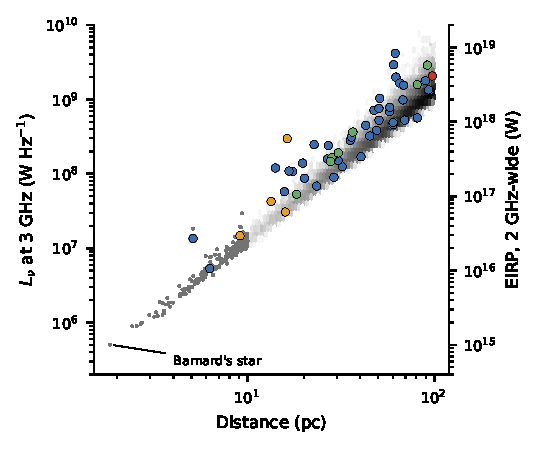
\includegraphics[width=0.6\textwidth]{vlass_perstar_limits.pdf}
\caption{95\% upper limits on the 3\,GHz spectral luminosity of individually undetected stars (grey) and luminosities of the secure associations (colors as in Figure~\ref{fig:cmd}) versus distance. The right axis gives the EIRP of a signal filling the 2\,GHz band.\label{fig:limits}}
\end{figure}

\begin{figure}
\centering
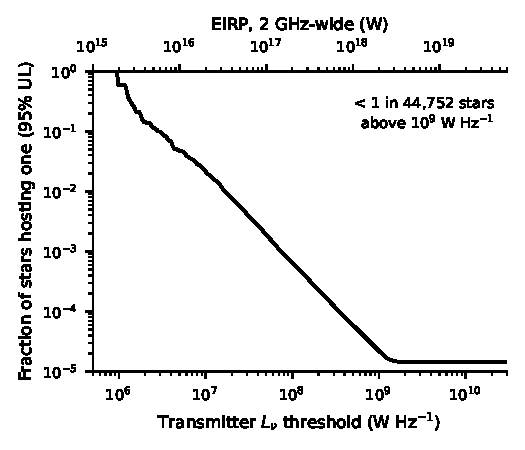
\includegraphics[width=0.6\textwidth]{vlass_population_limit.pdf}
\caption{95\% upper limit on the fraction of stars hosting a steady 2--4\,GHz transmitter above a given spectral luminosity (bottom axis) or 2\,GHz-wide EIRP (top axis), from individual non-detections. The curve flattens where all \NpopFloor\ stars contribute.\label{fig:pop}}
\end{figure}

\begin{deluxetable}{lrrrrr}
\tablecaption{95\% upper limits on steady 2--4\,GHz emission from the twelve nearest stars in the sample.\label{tab:nearest}}
\tablehead{\colhead{Star} & \colhead{$d$} & \colhead{$G_{BP}-G_{RP}$} & \colhead{$S_{\rm lim}$} & \colhead{$L_{\nu,\rm lim}$} & \colhead{EIRP$_{\rm lim}$} \\
\colhead{} & \colhead{(pc)} & \colhead{(mag)} & \colhead{(mJy)} & \colhead{(W\,Hz$^{-1}$)} & \colhead{(W)}}
\startdata
{Barnard's star} & 1.83 & 2.83 & 1.34 & $5.4\times10^{5}$ & $1.1\times10^{15}$ \\
{Wolf 359} & 2.41 & 4.18 & 1.25 & $8.7\times10^{5}$ & $1.7\times10^{15}$ \\
{HD 95735} & 2.55 & 2.22 & 1.23 & $9.6\times10^{5}$ & $1.9\times10^{15}$ \\
{G 272-61B} & 2.67 & 3.83 & 1.10 & $9.4\times10^{5}$ & $1.9\times10^{15}$ \\
{G 272-61A} & 2.72 & 3.75 & 1.10 & $9.7\times10^{5}$ & $1.9\times10^{15}$ \\
{CD-23 14742} & 2.98 & 2.83 & 1.27 & $1.3\times10^{6}$ & $2.7\times10^{15}$ \\
{Ross 248} & 3.16 & 3.53 & 1.06 & $1.3\times10^{6}$ & $2.5\times10^{15}$ \\
{eps Eri} & 3.22 & 1.14 & 1.17 & $1.4\times10^{6}$ & $2.9\times10^{15}$ \\
{HD 217987} & 3.29 & 2.10 & 0.92 & $1.2\times10^{6}$ & $2.4\times10^{15}$ \\
{Ross 128} & 3.37 & 3.03 & 1.36 & $1.9\times10^{6}$ & $3.7\times10^{15}$ \\
{61 Cyg B} & 3.50 & 1.72 & 0.85 & $1.2\times10^{6}$ & $2.5\times10^{15}$ \\
{61 Cyg A} & 3.50 & 1.46 & 0.85 & $1.2\times10^{6}$ & $2.5\times10^{15}$ \\
\enddata
\tablecomments{EIRP$_{\rm lim}=L_{\nu,\rm lim}\times2$\,GHz (band-filling signal).}
\end{deluxetable}


\subsection{Stacked emission} \label{sec:stacks}

Table~\ref{tab:stacks} and Figure~\ref{fig:stacks} present the stacks. The M-dwarf stacks show significant positive mean emission at 10--60\,pc, strongest at 20--40\,pc ($\StackMS\pm\StackMSerr\,\mu$Jy, \StackMSNR$\sigma$; median $\StackMMed\,\mu$Jy, \StackMMedSNR$\sigma$; $\langle\Lnu\rangle\approx\StackML\,\WHz$ from \StackMN\ stars). The signal is present in both halves of the sky and survives removal of the brightest 1\% of central pixels, so it is a property of the population rather than of a few sub-threshold flaring stars. Its amplitude is typical of quiescent emission from magnetically active M dwarfs \citep{GudelBenz1993,Callingham2021}. The apparent increase of $\langle\Lnu\rangle$ with distance is a selection effect: excluding individually detected stars removes the luminous tail of each shell above a threshold $\propto d^2$. No FGK stack exceeds \StackFGKmaxSNR$\sigma$.

\begin{figure*}
\centering
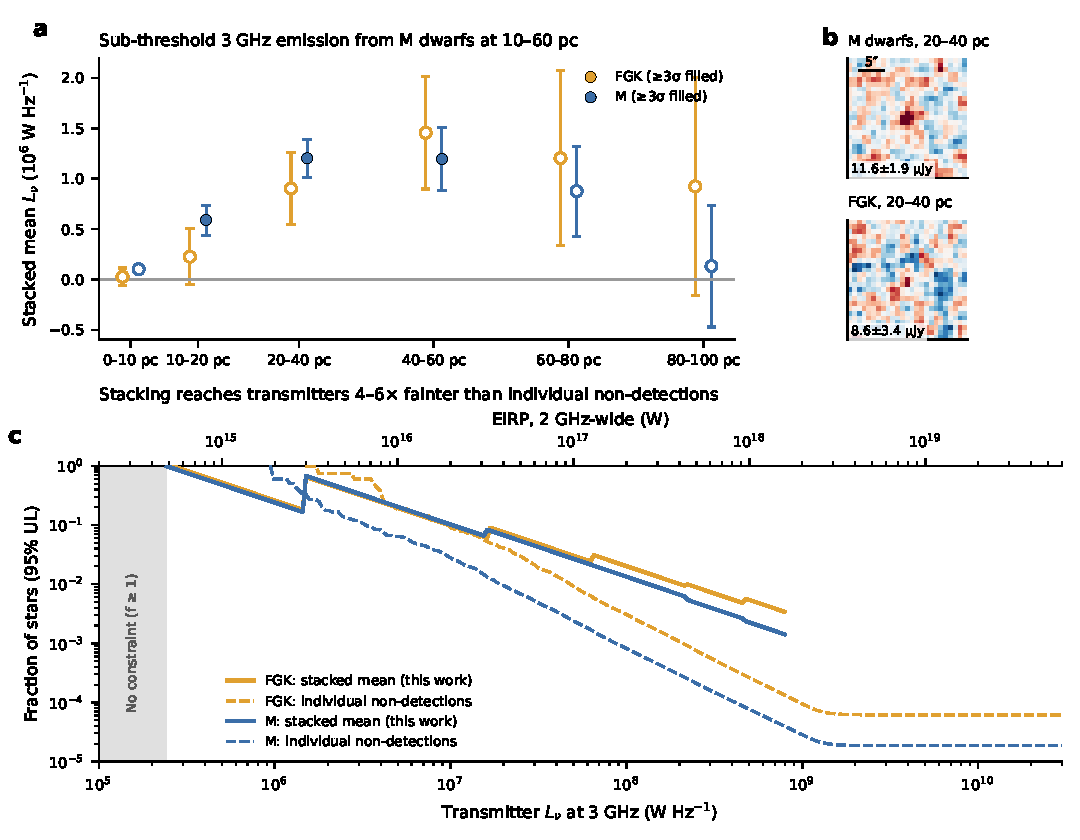
\includegraphics[width=0.95\textwidth]{vlass_ep1_stacking_summary.pdf}
\caption{(a) Inverse-variance-weighted mean 3\,GHz spectral luminosity of individually undetected stars in distance shells (filled: $\ge3\sigma$). (b) Flux-density stacks for M dwarfs and FGK stars at 20--40\,pc ($25''\times25''$). (c) 95\% upper limits on the fraction of stars hosting a transmitter of spectral luminosity $L_T$, from stacks (solid) and individual non-detections (dashed), cut at $f=1$; the shaded region is unconstrained by either method.\label{fig:stacks}}
\end{figure*}

\begin{deluxetable*}{llrrrrrrr}
\tablecaption{Inverse-variance-weighted mean stacks of VLASS Epoch 1 Quick Look images at the positions of individually undetected stars.\label{tab:stacks}}
\tablehead{\colhead{Shell} & \colhead{Type} & \colhead{$N$} & \colhead{$\langle S\rangle$} & \colhead{SNR} & \colhead{Median $S$} & \colhead{$\langle L_\nu\rangle$} & \colhead{$\langle L_\nu\rangle_{95}$} & \colhead{EIRP$_{95}$} \\
\colhead{(pc)} & \colhead{} & \colhead{} & \colhead{($\mu$Jy)} & \colhead{} & \colhead{($\mu$Jy)} & \colhead{($10^5$ W\,Hz$^{-1}$)} & \colhead{($10^5$ W\,Hz$^{-1}$)} & \colhead{(W)}}
\startdata
0--10 & FGK & 43 & $-6.9\pm24.4$ & $-0.3$ & $-5.5\pm31.1$ & $0.3\pm0.9$ & $1.7$ & $3.4\times10^{14}$ \\
0--10 & M & 161 & $33.1\pm13.2$ & $2.5$ & $27.6\pm15.5$ & $1.0\pm0.4$ & $1.6$ & $3.2\times10^{14}$ \\
10--20 & FGK & 314 & $7.0\pm10.4$ & $0.7$ & $5.5\pm12.8$ & $2.3\pm2.8$ & $6.8$ & $1.4\times10^{15}$ \\
10--20 & M & 1{,}221 & $25.2\pm6.1$ & $4.1$ & $16.1\pm6.2$ & $5.9\pm1.5$ & $8.3$ & $1.7\times10^{15}$ \\
20--40 & FGK & 2{,}691 & $8.6\pm3.4$ & $2.5$ & $8.2\pm4.2$ & $9.0\pm3.5$ & $14.8$ & $3.0\times10^{15}$ \\
20--40 & M & 9{,}864 & $11.6\pm1.9$ & $6.2$ & $11.8\pm2.2$ & $12.0\pm1.9$ & $15.2$ & $3.0\times10^{15}$ \\
40--60 & FGK & 7{,}697 & $4.6\pm1.9$ & $2.4$ & $5.2\pm2.4$ & $14.6\pm5.6$ & $23.7$ & $4.7\times10^{15}$ \\
40--60 & M & 25{,}549 & $3.8\pm1.1$ & $3.6$ & $2.2\pm1.3$ & $11.9\pm3.1$ & $17.1$ & $3.4\times10^{15}$ \\
60--80 & FGK & 14{,}165 & $2.0\pm1.5$ & $1.4$ & $-0.3\pm1.8$ & $12.0\pm8.7$ & $26.3$ & $5.3\times10^{15}$ \\
60--80 & M & 47{,}343 & $1.6\pm0.8$ & $2.1$ & $2.0\pm0.9$ & $8.8\pm4.5$ & $16.1$ & $3.2\times10^{15}$ \\
80--100 & FGK & 23{,}143 & $1.0\pm1.1$ & $0.9$ & $1.5\pm1.4$ & $9.2\pm10.8$ & $27.0$ & $5.4\times10^{15}$ \\
80--100 & M & 75{,}220 & $0.1\pm0.6$ & $0.2$ & $0.6\pm0.8$ & $1.3\pm6.0$ & $11.3$ & $2.3\times10^{15}$ \\
\enddata
\tablecomments{Means are measured against the empirical null (stacked image at 10--18$''$ from the centre); uncertainties are the larger of the formal and null-ring scatter. $\langle L_\nu\rangle_{95}$ is the one-sided 95\% upper limit on the mean spectral luminosity; EIRP$_{95}$ assumes a flat signal filling 2\,GHz. FGK/M split at $G_{BP}-G_{RP}=1.84$.}
\end{deluxetable*}


Treating the entire stacked signal as potentially artificial, the stacks limit transmitters 4--6 times fainter than the individual non-detections (Figure~\ref{fig:stacks}c): the constraint reaches $f<1$ at $L_T=\ReachFGK\,\WHz$ for FGK stars and $\ReachM\,\WHz$ for M dwarfs, compared with $\DetReachFGK$ and $\DetReachM\,\WHz$ from individual non-detections, and at $L_T=10^6\,\WHz$ gives $f<\FStackSixFGK$ (FGK) and $f<\FStackSixM$ (M). Above $\sim10^7\,\WHz$ the individual limits are more constraining. Because natural emission is detected in the M-dwarf stacks, their limits are conservative.

\section{Discussion} \label{sec:discussion}

\subsection{Comparison with narrowband searches} \label{sec:bl}

Table~\ref{tab:bl} compares our limits for a star at 50\,pc with those of \citet{Price2020}, whose GBT and Parkes bands overlap VLASS at 2.0--2.8 and 2.6--3.45\,GHz. In flux density VLASS is $\sim\FluxRatio$ times deeper (\VlassFiftyS\,mJy against $\approx$7\,Jy), because it integrates over 2\,GHz rather than a 2.79\,Hz channel. For a narrow line, however, the continuum dilutes the power over the band, and our in-band EIRP limit ($\VlassFiftyEIRP$\,W) is $\sim\BLratio$ times higher than the BL limit of $2.1\times10^{12}$\,W. For a signal of bandwidth $B$, the sensitivity of a single narrowband channel degrades roughly as $B$, whereas the continuum limit is independent of $B$: the two cross near $B\sim300$\,kHz, and for broader signals---radar chirps, spread-spectrum links, or broadband leakage---the continuum survey is the more sensitive, while the turboSETI pipeline used by \citet{Price2020} does not detect such signals at all. In occurrence, the continuum survey's large sample gives $f<\FFifty$ for the \NFifty\ stars within 50\,pc ($\FFiftyHalf$ with the 50\% detection probability adopted by \citealt{Price2020}), about 20 times tighter than the 0.37--0.45\% GBT narrowband limits under the same assumption, albeit at an EIRP threshold five orders of magnitude higher. The two approaches are complementary: narrowband searches constrain faint, narrow, long-duty-cycle signals around $\sim10^3$ stars, and continuum surveys constrain bright, broad signals around $\sim10^5$.

\begin{deluxetable*}{llllrr}
\tablecaption{Comparison with the Breakthrough Listen narrowband survey of \citet{Price2020} for a star at 50\,pc.\label{tab:bl}}
\tablehead{\colhead{Survey} & \colhead{Band} & \colhead{Dwell} & \colhead{$S_{\rm lim}$ (Jy)} & \colhead{EIRP$_{\rm lim}$ (W)} & \colhead{$N_\star$}}
\startdata
BL GBT & 1.10--2.80 GHz & $3\times5$ min ON & $7.0$ & $2.1\times10^{12}$ & 882 \\
BL Parkes & 2.60--3.45 GHz & multi-epoch & $3.0\times10^{1}$ & $9.1\times10^{12}$ & 189 \\
This work (VLASS QL) & 2--4 GHz & $\sim$5 s snapshots & $5.6\times10^{-4}$ & $3.3\times10^{17}$ & 26{,}741 \\
\enddata
\tablecomments{Breakthrough Listen (BL) limits apply to signals $\lesssim$3\,Hz wide with $|\dot\nu|\le4$\,Hz\,s$^{-1}$ and use the 1\,Hz transmitter-width convention of \citet{Price2020}; the VLASS limit applies to the total in-band power of any signal. $N_\star$ is the number of stars constraining the occurrence limit (for VLASS: stars within 50\,pc).}
\end{deluxetable*}


Figure~\ref{fig:tr} places these limits in the plane of transmitter rate against EIRP$_{\rm min}$ used to compare technosignature surveys \citep{Enriquez2017,Price2020,Painter2025}. The transmitter rate is $(N_\star\,\nu_{\rm rel})^{-1}$, where $\nu_{\rm rel}=\Delta\nu/\nu_c$ is the fractional bandwidth, 2/3 for VLASS. Because our population limit at a given EIRP involves only the $N_{\rm eff}$ stars individually sensitive to it, the VLASS limit is a curve rather than a point. It falls from $\approx0.5$ at $2\times10^{15}$\,W to $\TRfloor$ above $\sim3\times10^{18}$\,W, where all \NpopFloor\ stars contribute. For the stacks, which limit a fraction rather than count stars, we use the equivalent number $N=3/f_{95}$ and show them only where they are more constraining than the individual limits. The VLASS floor is lower than the transmitter rate reached by any of the surveys shown with EIRP$_{\rm min}<10^{20}$\,W, but the comparison is not like for like. The narrowband EIRP$_{\rm min}$ values assume a 1\,Hz-wide transmitter and include the factor of 3.3 correction of \citet{Choza2024}, whereas the VLASS values are the total in-band power and apply to a signal of any bandwidth.

\begin{figure*}
\centering
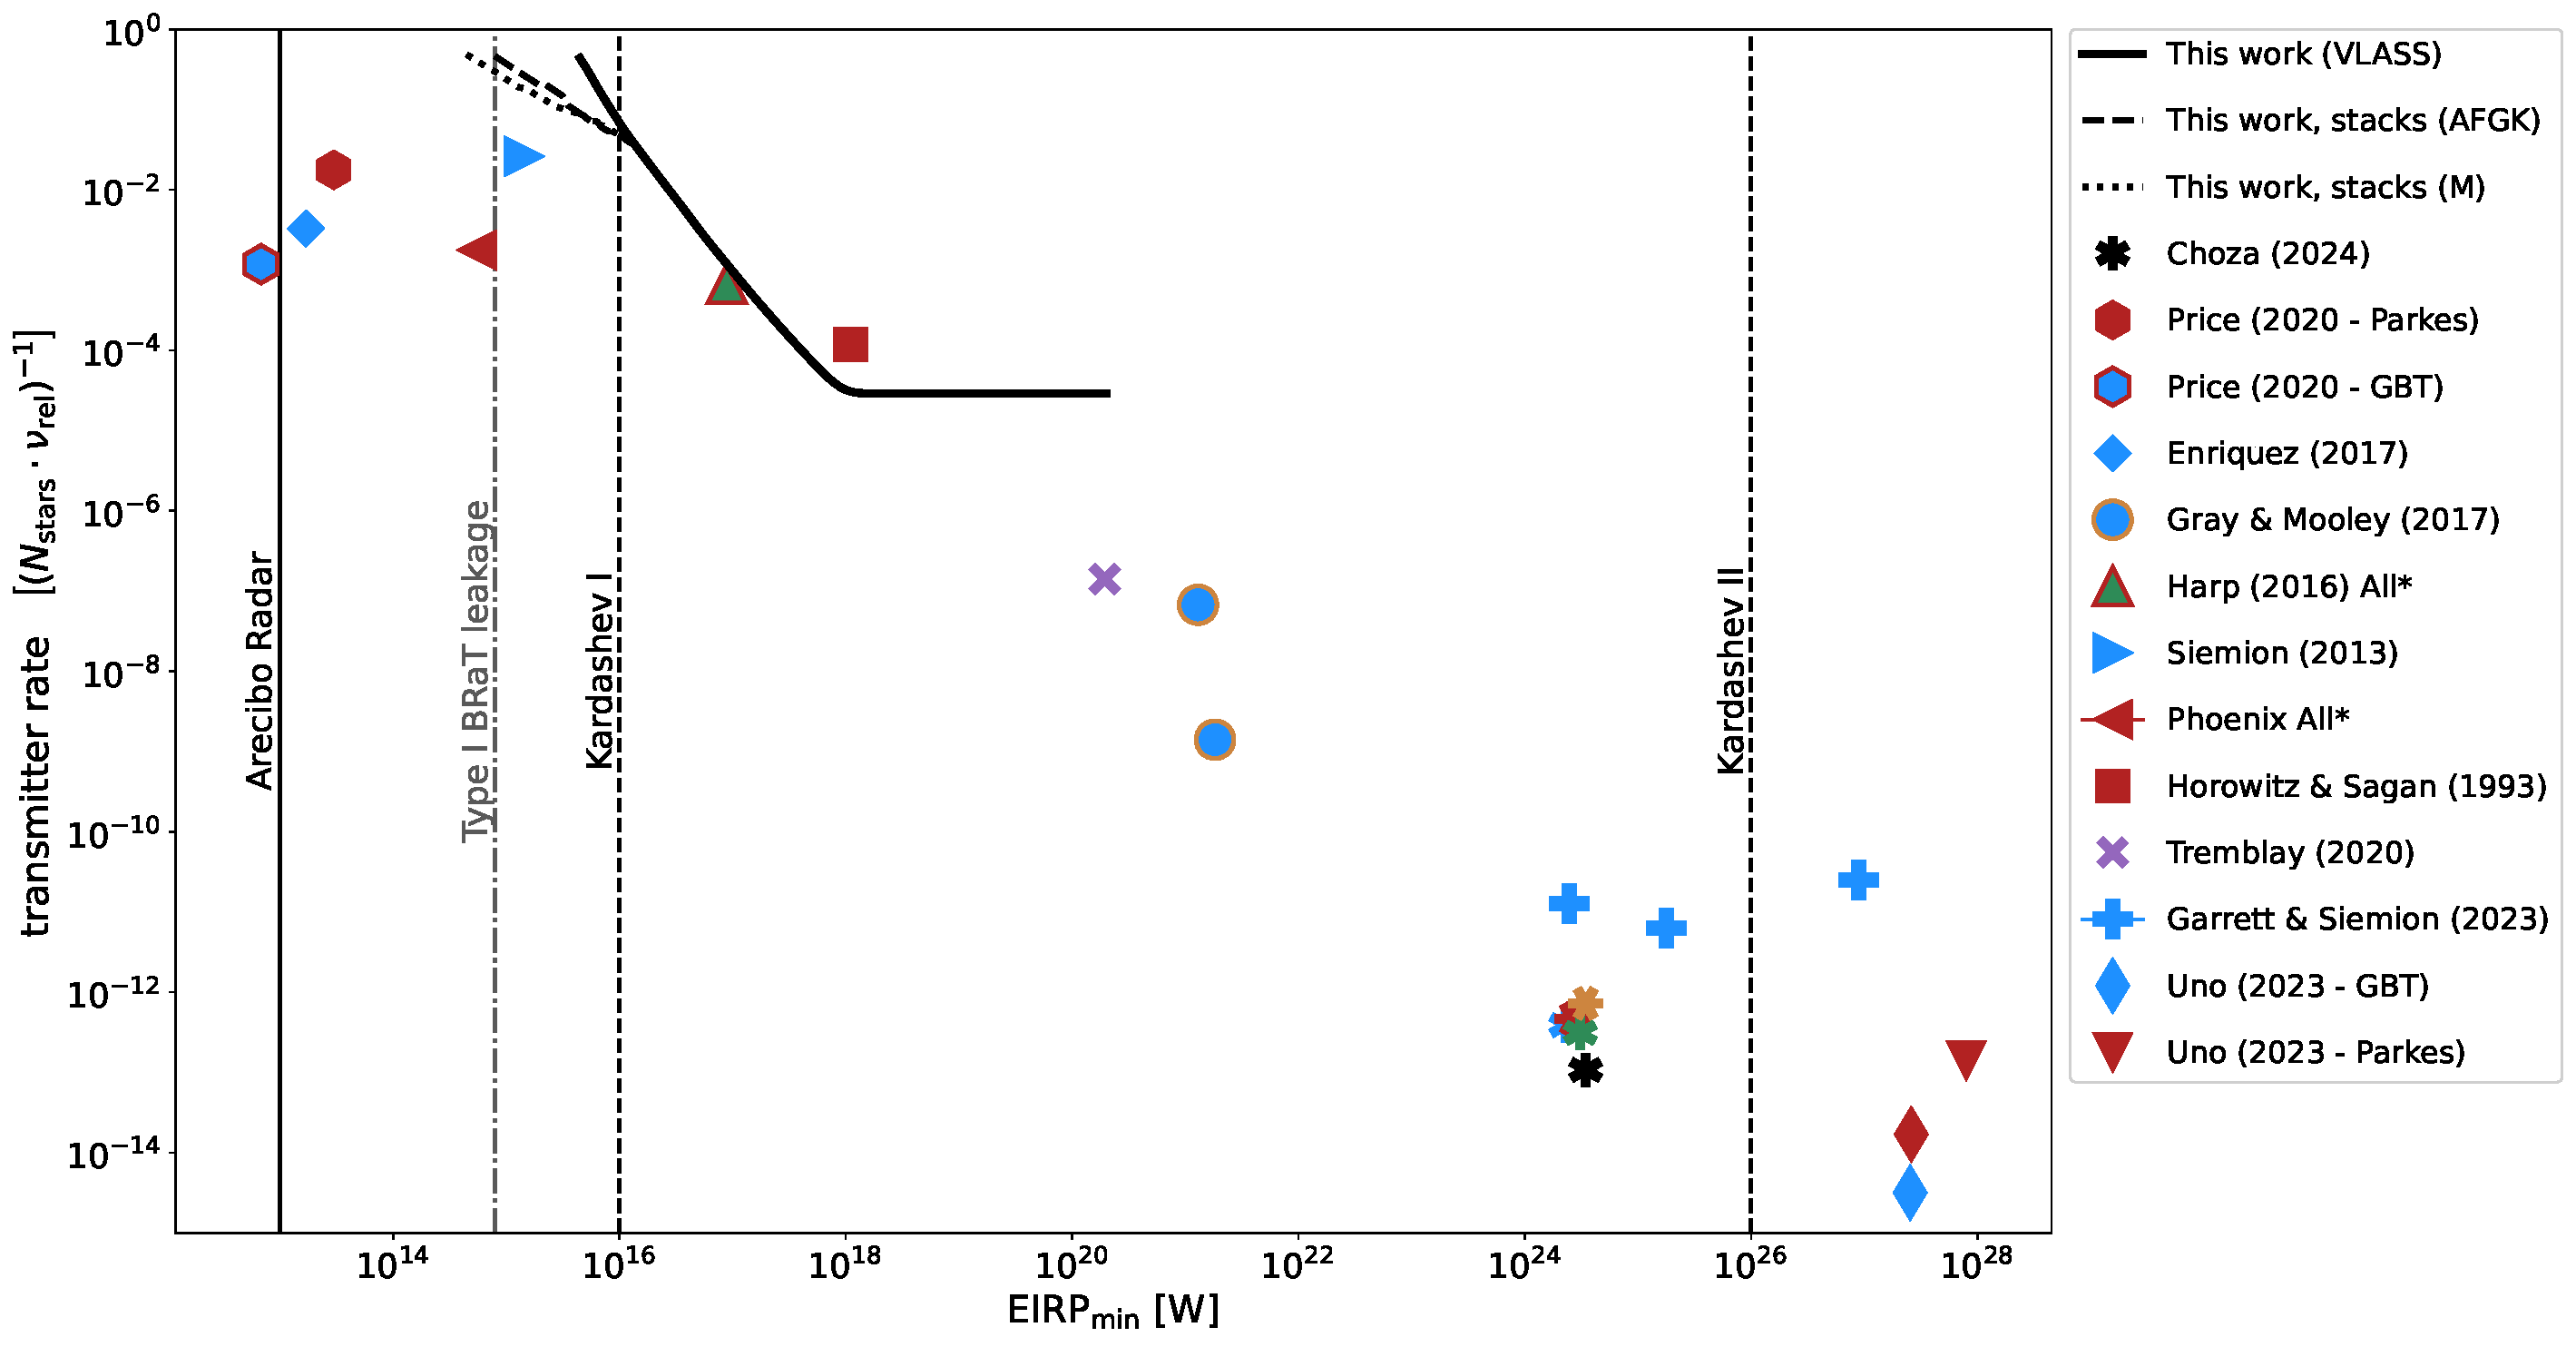
\includegraphics[width=\textwidth]{transmitter_rate_vs_eirp.pdf}
\caption{Transmitter rate versus EIRP$_{\rm min}$ for this work and for previous radio technosignature surveys \citep{HorowitzSagan1993,Backus2004,Siemion2013,Harp2016,Enriquez2017,GrayMooley2017,Price2020,TremblayTingay2020,Garrett2022,Uno2023,Choza2024}, following \citet[their Figure~15]{Painter2025}; literature values are plotted with the compilation of B.~Jacobson-Bell (in preparation). Narrowband limits assume 1\,Hz-wide transmitters and are corrected following \citet{Choza2024}. VLASS limits (black) are for the total in-band power of a signal of any width: individual non-detections (solid) and, where more constraining, the FGK (dashed) and M-dwarf (dotted) stacks. Vertical lines mark the EIRP of the Arecibo radar, the Kardashev Type~I and II power levels, and the Type~I broadband leakage benchmark of \citet{Garrett2026} spread over 2\,GHz.\label{fig:tr}}
\end{figure*}


\subsection{Comparison with broadband leakage benchmarks} \label{sec:brats}

Treating the band-averaged 3\,GHz luminosity as representative of a flat broadband spectrum, the Type~I leakage benchmark of \citet{Garrett2026}, $\Lnu\sim4\times10^5\,\WHz$ (EIRP $\approx8\times10^{14}$\,W across 2\,GHz), lies just below our most sensitive individual limit, $\Lnu<\BarnardL\,\WHz$ for Barnard's star; no star in the sample is individually constrained at that level. The stacks do reach it: at $4\times10^5\,\WHz$ they require $f<\FBratFGK$ for FGK stars and $f<\FBratM$ for M dwarfs, a weak but direct constraint on the prevalence of such leakage among nearby stars. Earth's present aggregate leakage of $\sim400\,\WHz$ would be detectable at the median VLASS sensitivity only to $\sim\EarthLeakAU$\,AU. Several of the diagnostics proposed by \citet{Garrett2026} are out of reach at VLASS resolution and depth---brightness temperature, polarization, spectral structure, and scintillation---but two are central to this work: association with a Gaia star, and co-motion with it (Section~\ref{sec:lspm}). A BRaT from a planet would be offset from its host by $\lesssim0.1''$ for orbits of a few AU at $d\gtrsim30$\,pc, well within our matching tolerance. Frequencies $\gtrsim1$\,GHz also avoid the elevated ionospheric cut-off expected for planets around active M dwarfs \citep{Garrett2026}, which favors 2--4\,GHz for the M dwarfs that make up most of our sample.

\subsection{Interpretation and caveats} \label{sec:caveats}

Our limits apply to emission that is on during the few-second VLASS snapshot, Stokes~I, and within the 2--4\,GHz band (excluding subbands flagged for radio-frequency interference). The EIRP values assume a flat, band-filling spectrum; for a signal occupying a fraction of the band the EIRP limit is unchanged, but the spectral-luminosity limit applies to the band-averaged power. Positions neglect parallax, and our image noise estimate (the mean island rms of each image) is slightly conservative. The main-sequence selection includes unresolved binaries; the classification of natural emitters relies in part on SIMBAD, a live database. Finally, a technosignature co-located with a natural emitter cannot be excluded below the natural emission level; for the \NDetected\ detected stars our limit is the measured flux density.

\subsection{Prospects} \label{sec:prospects}

VLASS Epochs 2 and 3, already available at CADC, will deepen the stacks by $\sqrt3$ and sample the transmitter duty cycle at three epochs, and Single Epoch imaging improves the flux scale and astrometry. Multi-epoch astrometry, as applied here to LSPM~J1943+5337, provides a general and decisive test for any future candidate around a high-proper-motion star. Lower-frequency continuum surveys extend the method to where coherent stellar emission and many terrestrial transmitters are strongest \citep{Callingham2021}, and the same approach applies to background sources behind BL targets \citep{Garrett2022} and to other stellar objects in survey fields \citep{Wlodarczyk2020}.

\section{Conclusions} \label{sec:conclusions}

We searched \NSample\ main-sequence stars within 100\,pc for excess 2--4\,GHz continuum emission in VLASS Epoch~1. Of \NSecure\ secure associations, \NNatural\ are known natural emitters, and the remaining source, near LSPM~J1943+5337, is a background source that does not share the star's proper motion. We place 95\% limits on steady broadband emission from every star---median $\Lnu<\LlimMed\,\WHz$ and $\Lnu<\BarnardL\,\WHz$ for Barnard's star---and on the transmitter fraction, $f<\FpopNine$ above $10^9\,\WHz$. Stacking reveals natural sub-threshold M-dwarf emission and extends population constraints 4--6 times fainter than individual non-detections. Continuum surveys are a sensitive, modulation-agnostic complement to narrowband technosignature searches.

\section{Data availability} \label{sec:data_avail}

All code, the downloaded catalogs, the \NCutouts\ VLASS cutouts, and the derived tables and figures are available at Zenodo (TODO: DOI). Each script records the exact query used, and the package reproduces every number in this paper.

\begin{acknowledgments}

S.C. is supported by funding from Breakthrough Listen. The Breakthrough Prize Foundation funds the Breakthrough Initiatives, which manages Breakthrough Listen.

The National Radio Astronomy Observatory is a facility of the National Science Foundation operated under cooperative agreement by Associated Universities, Inc. CIRADA is funded by a grant from the Canada Foundation for Innovation 2017 Innovation Fund (Project 35999), as well as by the Provinces of Ontario, British Columbia, Alberta, Manitoba and Quebec. This research used the facilities of the Canadian Astronomy Data Centre operated by the National Research Council of Canada with the support of the Canadian Space Agency. This work has made use of data from the European Space Agency (ESA) mission Gaia, processed by the Gaia Data Processing and Analysis Consortium (DPAC). Funding for the DPAC has been provided by national institutions, in particular the institutions participating in the Gaia Multilateral Agreement. This research has made use of the SIMBAD database and the VizieR catalogue access tool, CDS, Strasbourg, France, accessed via the CfA mirrors. The Digitized Sky Surveys were produced at the Space Telescope Science Institute under U.S. Government grant NAG W-2166. The Pan-STARRS1 Surveys have been made possible through contributions by the institutions listed in \citet{Chambers2016}.

Analysis code and an initial draft of this manuscript were prepared with assistance from an AI system (Claude Opus 5.5, Anthropic); all results were verified by the author.
\end{acknowledgments}

%% Facility keywords from the AAS list (journals.aas.org/facility-keywords). PO:1.2m = Samuel Oschin Schmidt (POSS-I/II plates, via DSS);
%% MAST served the DSS and PS1 data. CADC (VLASS images) is acknowledged in the text; add it here if it appears in the AAS list.
\facilities{VLA, Gaia, ROSAT, eROSITA, PS1, PO:1.2m, MAST}

\software{Astropy \citep{Astropy2013,Astropy2018,Astropy2022}, NumPy \citep{Harris2020}, SciPy \citep{Virtanen2020}, pandas \citep{McKinney2010}, Matplotlib \citep{Hunter2007}, PyVO \citep{Graham2014}}






\clearpage
\bibliography{refs}{}
\bibliographystyle{aasjournalv7.1_patched}

\end{document}
